\section{Situación Problemática}

\label{sec:SituacionProblematica}

Los glaciares, formaciones de hielo ubicadas en regiones montañosas y polares, son componentes vitales del sistema climático terrestre. Actúan como reservorios naturales de agua dulce y son indicadores clave del cambio climático, ya que sus fluctuaciones de crecimiento o desaparición reflejan las variaciones en las condiciones climáticas \cite{johansen2019atlas}. Sin embargo, el calentamiento global ha provocado un retroceso significativo de los glaciares en varias regiones, lo que plantea un desafío crítico para la conservación de estos ecosistemas y la protección de los recursos hídricos que proveen \cite{ali2023intimidating, rounce2023global}.

La Organización de las Naciones Unidas para la Educación, la Ciencia y la Cultura (UNESCO) estima que aproximadamente 58.000 millones de toneladas de hielo se desvanecen anualmente, contribuyendo al 5\% del incremento del nivel del mar \cite{carvalho2022world}. Este fenómeno representa graves repercusiones ambientales y socioeconómicas a nivel local y mundial \cite{mark2017glacier, nie2021glacial, clague2023impacts}. Entre los efectos más evidentes están la alteración de los ciclos hidrológicos, la reducción de la disponibilidad de agua dulce para consumo humano, agricultura y generación de energía hidroeléctrica, y el incremento en el riesgo de desastres naturales como inundaciones, deslizamientos de tierra y avalanchas \cite{motschmann2020losses}. Además, la pérdida de glaciares tiene un impacto directo en la biodiversidad de los ecosistemas de montaña y áreas adyacentes, lo que puede llevar a la degradación de los ecosistemas y la posible extinción de especies endémicas \cite{palomo2017climate}. Desde un enfoque socioeconómico, la retracción glaciar tiene un impacto adverso en el turismo, la pesca y las comunidades que dependen de estos recursos naturales para su subsistencia \cite{rasul2019global}.

La Cordillera de los Andes, una de las cadenas montañosas más extensas del mundo con presencia de glaciares, se extiende por todo el continente sudamericano, atravesando países como Venezuela, Colombia, Ecuador, Perú, Bolivia, Chile y Argentina \cite{johansen2019atlas}. Esta cordillera alberga aproximadamente el 99\% de los glaciares tropicales, situándose como la región con la mayor concentración de estos ecosistemas a nivel mundial \cite{veettil2019global}.

\begin{figure}[H]
    \begin{center}
        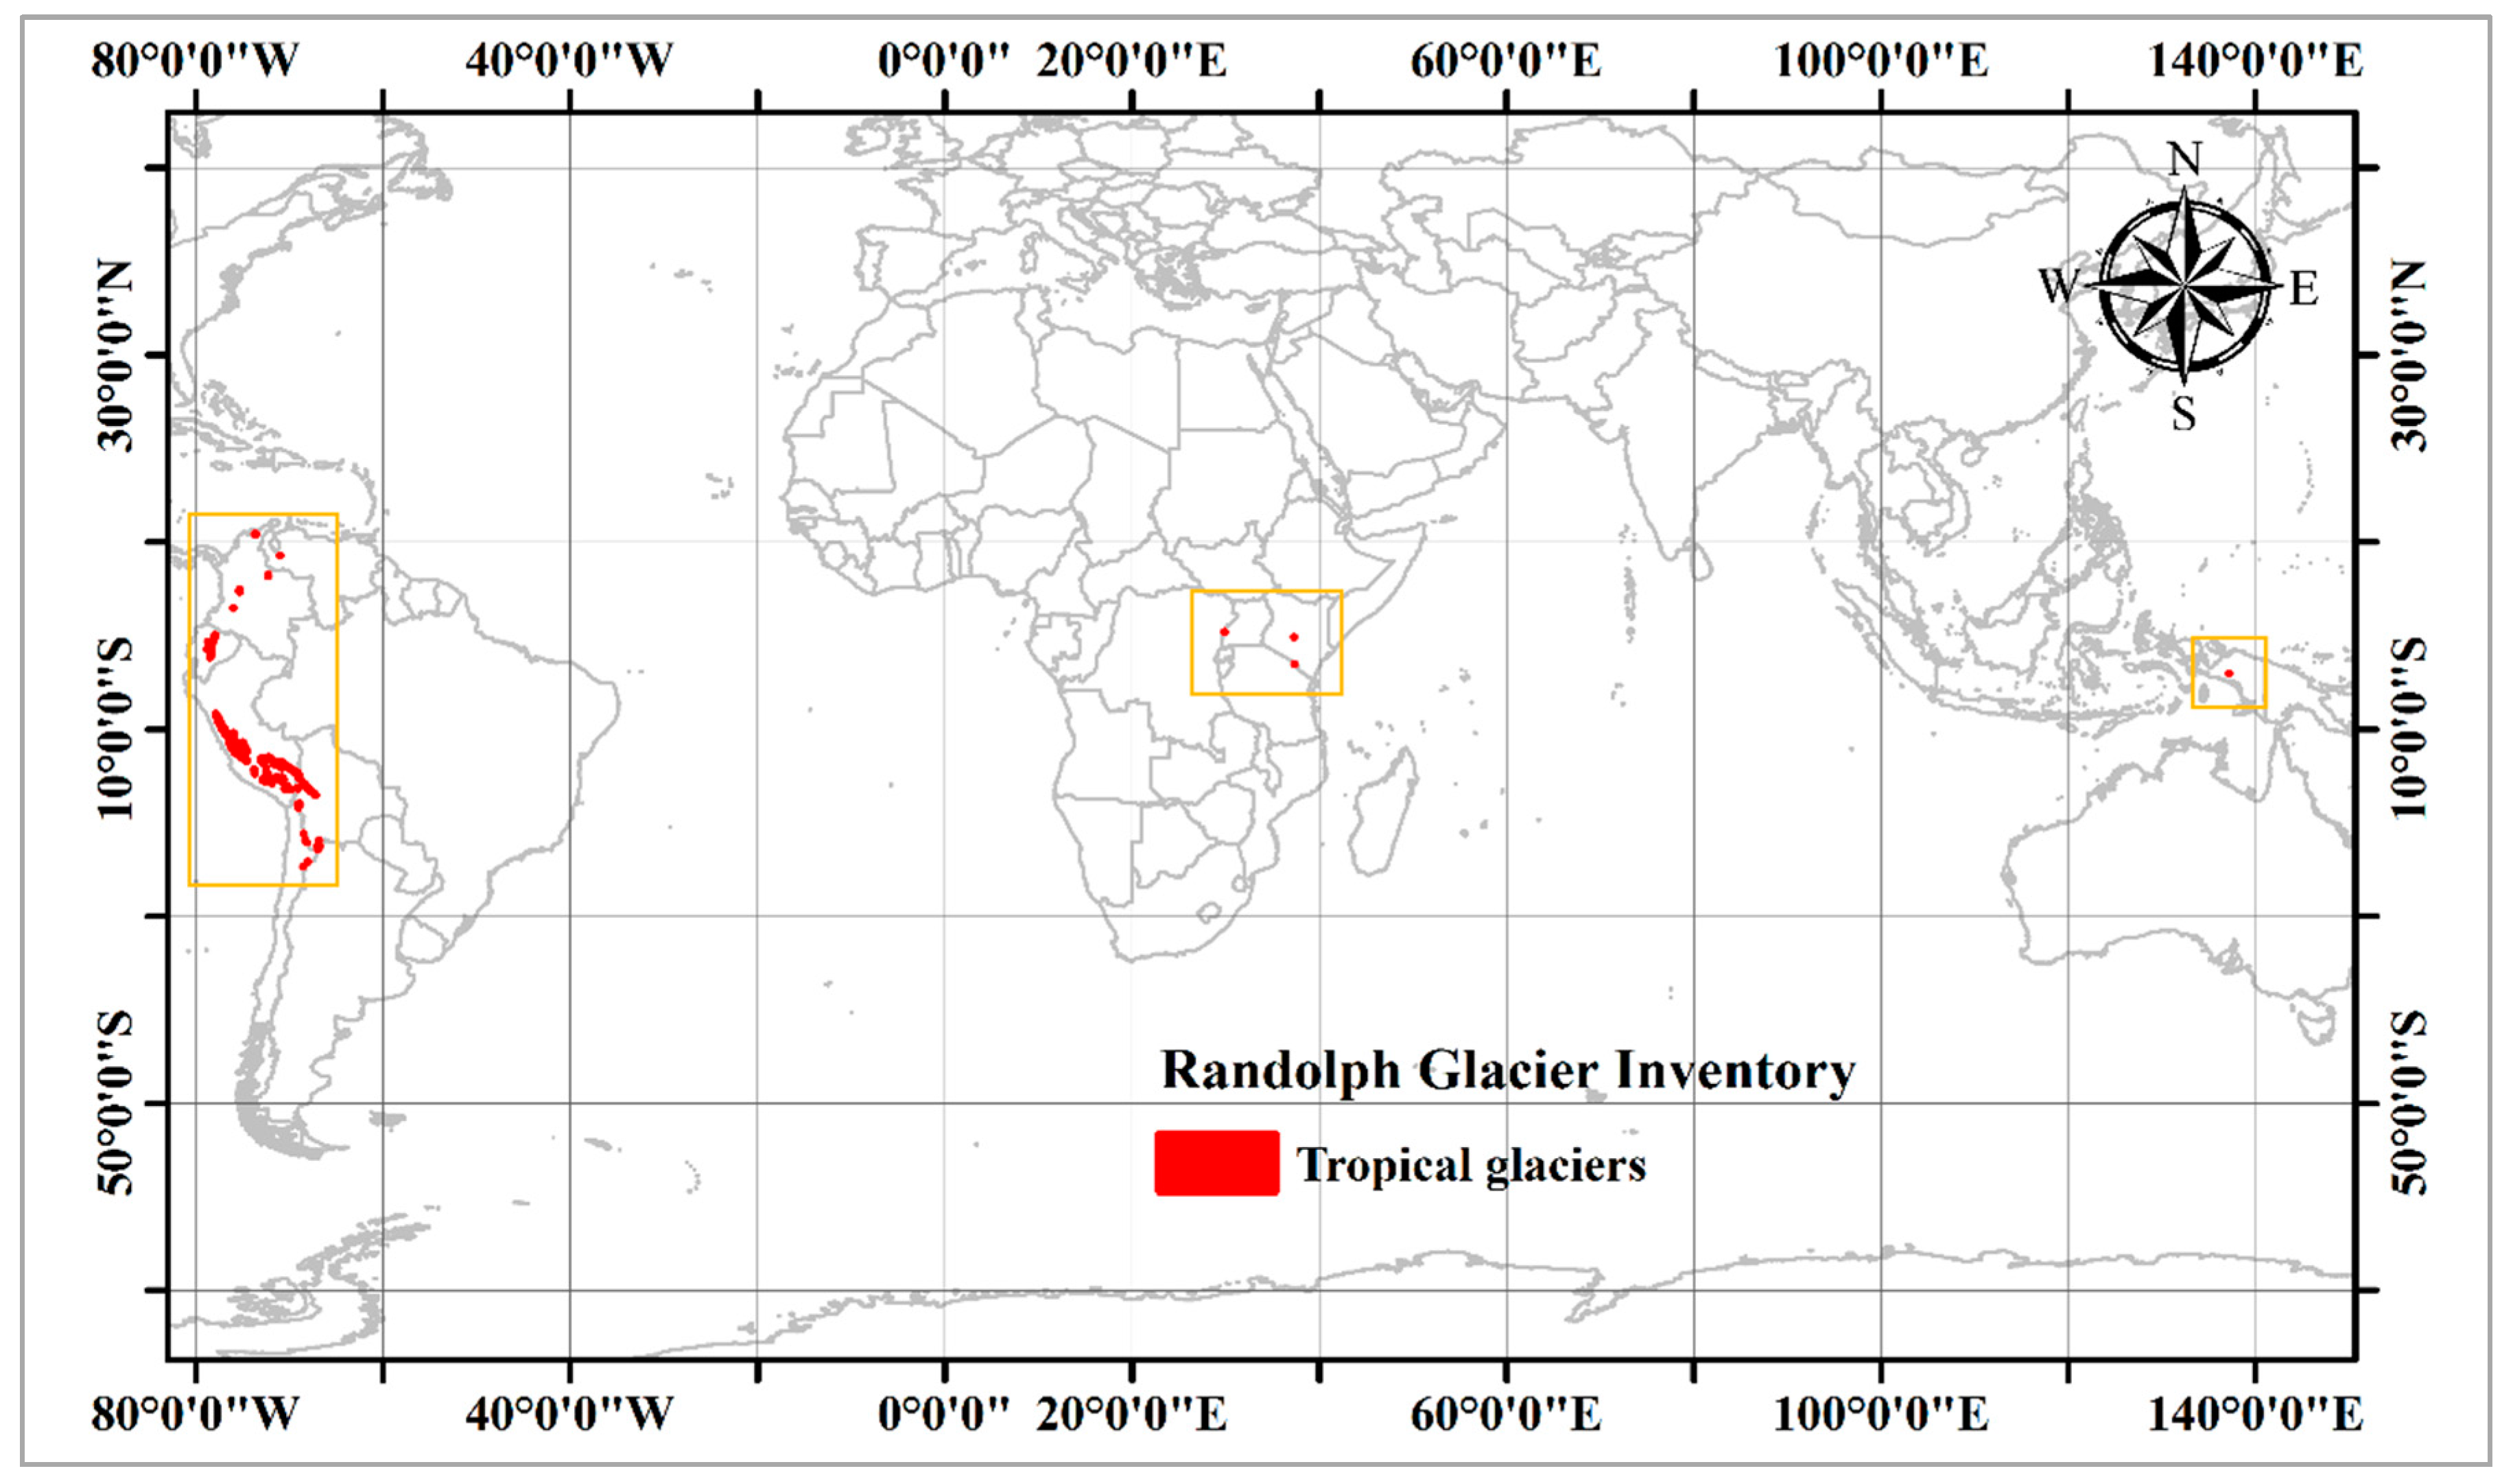
\includegraphics[width=1\textwidth]{Images/GlaciaresTropicales.png}
    \end{center}
    \caption{Distribución geográfica de los glaciares tropicales alrededor del mundo.}
    \reference{Datos tomados de \citeA{veettil2019global}.}
    \label{fig:GlaciaresTropicales}
\end{figure}

Los glaciares tropicales se denominan así debido a su ubicación cercana a la línea ecuatorial, entre el Trópico de Cáncer y el Trópico de Capricornio ($23^\circ 26'13.3'' \text{ N}$; $23^\circ 26'13.3'' \text{ S}$) (ver Figura~\ref{fig:GlaciaresTropicales}). Su ubicación los hace especialmente sensibles a las fluctuaciones climáticas, siendo incluso más susceptibles al calentamiento global que sus contrapartes en regiones polares \cite{dussaillant2019two}. Perú es el país con mayor presencia de glaciares tropicales en el mundo. Según datos del Randolph Glacier Inventory \cite{pfeffer2014randolph}, recopilados por \cite{veettil2019global}, cuenta con un total aproximado de 1602,96 km$^2$ de glaciares tropicales, lo que representa el 68.38\% del total a nivel mundial. Sin embargo, en los últimos 50 años, la superficie glaciar en el territorio peruano se ha reducido en un 53\% \cite{reserva2021}.

El Instituto Nacional de Investigación en Glaciares y Ecosistemas de Montaña (INAIGEM) es el órgano responsable del estudio y monitoreo de los glaciares y ecosistemas de montaña en Perú, y es la entidad encargada de la elaboración del Inventario Nacional de Glaciares \cite{inaigem2018inventario}.

Los inventarios de glaciares son instrumentos que forman parte de las políticas de diversos países para responder a las problemáticas relacionadas al deterioro de los ecosistemas de montaña \cite{barella2022combined}. Un inventario de glaciares proporciona información detallada del estado actual de los glaciares de una región específica a través de la recopilación de datos históricos, la delimitación y categorización de la superficie glaciar, y el posterior análisis para la elaboración de modelos predictivos que permitan identificar posibles acciones estratégicas para su conservación a través de una correcta toma de decisiones \cite{barcaza2017glacier}.

La recopilación de datos relacionados a los ecosistemas de montaña siempre se ha considerado una tarea compleja debido al difícil acceso provocado por las condiciones climáticas extremas propias del entorno y los limitados medios de transporte \cite{fang2017discriminative, nijhawan2018hybrid}. Sin embargo, la emergencia de datos provenientes de sensores remotos, en particular, las imágenes satelitales y otros productos derivados, ha simplificado significativamente este proceso \cite{gavade2021systematic}.

La implementación de técnicas de teledetección ha impulsado numerosos estudios, facilitando la adquisición y el posterior procesamiento de la información recopilada \cite{zhang2019glacier}. Entre las distintas estrategias utilizadas para esta última etapa, resalta el uso de índices espectrales. Un ejemplo notable es el Índice Normalizado de Diferencia de Nieve (NDSI, por sus siglas en inglés), el cual permite identificar las áreas cubiertas de nieve \cite{hall1995mapping}. Esto se logra mediante la diferencia normalizada entre una banda visible y una banda cercana al infrarrojo o infrarrojo de onda corta del espectro en una imagen satelital multiespectral \cite{hall2010normalized}. Además, se complementa con la definición de umbrales de valor y, en algunos casos, la discriminación visual de los resultados \cite{sibandze2014comparison, singh2021quantifying}. Países como Perú, Chile, Argentina y Colombia, han adoptado estas técnicas para la delimitación de la superficie glaciar, complementándolas con datos adicionales como modelos digitales de elevación e imágenes de alta resolución \cite{inaigem2017manual, DGA2022, castro2014manual, ospina2022metodologia}.

Aunque los métodos tradicionales han mostrado eficacia en la delimitación de la superficie glaciar, presentan algunas desventajas, como la tendencia a sobre estimar los resultados y una fuerte dependencia de la intervención humana debido a las limitaciones inherentes de la información espectral \cite{singh2021quantifying}.

La información espectral de una imagen satelital se deriva de la reflectancia de la superficie terrestre, que es la fracción de energía solar reflejada por la superficie y captada por los sensores del satélite \cite{chuvieco2016fundamentals}. Sin embargo, aunque este proceso es efectivo para identificar cuerpos de nieve limpios, puede verse afectado por diversos factores, como la atmósfera, la topografía, la vegetación, la nieve estacionaria, y las propiedades físicas del suelo, lo que puede generar errores en la interpretación de los datos \cite{lu2020glacier, tian2022mapping}.

Además de los desafíos previamente mencionados, surge la necesidad de identificar otros tipos de glaciares, como los glaciares cubiertos y los glaciares rocosos, los cuales presentan desafíos únicos debido a sus características particulares (ver Figura \ref{fig:ComparacionGlaciares}). Los glaciares cubiertos, tal y como su nombre lo indica, están recubiertos por una capa de escombros o rocas que pueden alterar significativamente su firma espectral, dificultando su identificación mediante métodos de teledetección tradicionales debido a su similitud con el terreno circundante \cite{zhang2019glacier}. Los glaciares rocosos, por otro lado, son glaciares compuestos por una mezcla de hielo y rocas, que al igual que los glaciares cubiertos, comparten la misma dificultad en su proceso de identificación \cite{robson2020automated}.

\begin{figure}[H]
    \begin{center}
        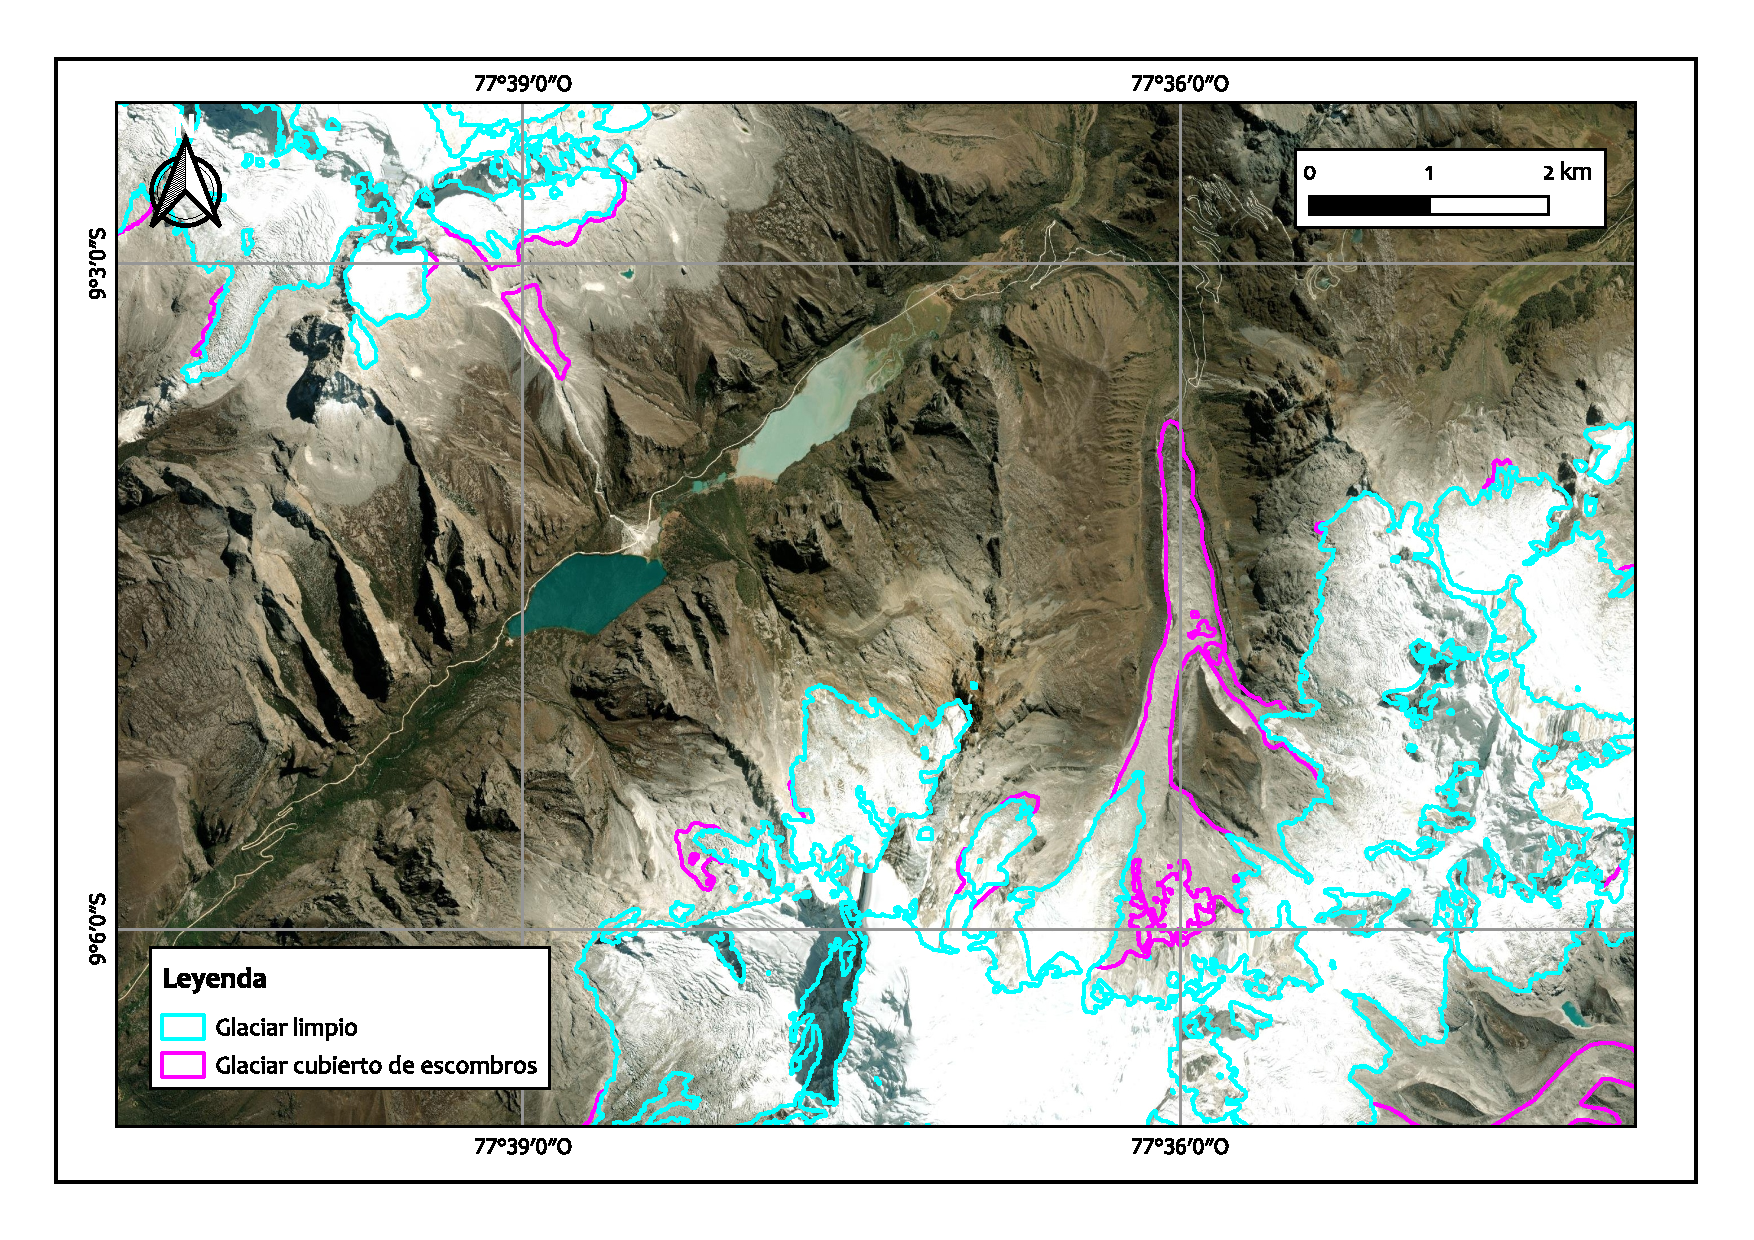
\includegraphics[width=1\textwidth]{Images/ComparacionGlaciares.pdf}
    \end{center}
    \caption{Diferencias visuales entre un glaciar limpio y un glaciar cubierto de escombros.}
    \reference{Elaborado por el autor.}
    \label{fig:ComparacionGlaciares}
\end{figure}

La importancia de la identificación de estos tipos de glaciares radica en su impacto sobre las tasas de derretimiento glaciar \cite{lu2021novel}. Los escombros delgados tienden a acelerar el derretimiento, mientras que los escombros más gruesos lo ralentizan \cite{anderson2021causes}. Además, la presencia de glaciares cubiertos también puede indicar reservas potenciales de recursos hídricos, ya que estos no están expuestos directamente a la atmósfera y por tanto, pueden retener agua de forma más efectiva \cite{zhang2019role, florath2021optical}.

Dada su semejanza espectral con el terreno circundante, la identificación de estos tipos de glaciares puede resultar en sobre estimaciones y errores en la delimitación \cite{nijhawan2018hybrid}. Los métodos tradicionales intentan abordar este desafío a través de una delimitación manual, que se basa en el uso de información adicional como imágenes de alta resolución y la obtención de parámetros morfométricos a partir de modelos digitales de elevación e imágenes satelitales de radar \cite{fang2017discriminative, lu2020glacier}. A pesar de su utilidad, este enfoque requiere una gran cantidad de experticia, y es un proceso lento, laborioso y sujeto a errores, principalmente debido a la subjetividad de la evaluación \cite{yan2021glacier, zhang2021automated, xie2022progressive, hu2022new}.

Frente a estos desafíos, las técnicas alternativas han ido ganando terreno en el ámbito de la delimitación de glaciares, destacándose en particular el Análisis de Imágenes Basado en Objetos (OBIA) y el Análisis de Imágenes Basado en Píxeles (PBIA) \cite{muhammad2013comparison, rastner2013comparison}. Sin embargo, entre estas nuevas propuestas, las técnicas que incorporan Inteligencia Artificial (IA) están cobrando una relevancia notable, gracias a su rendimiento en disciplinas de teledetección tan variadas como la agricultura, la gestión forestal y los estudios marítimos, por mencionar algunos \cite{hoeser2020object2}. Además, estas técnicas ofrecen una solución al manejo de la creciente cantidad de datos disponibles, al ser capaces de procesar grandes volúmenes de información, superando una limitación importante de los métodos tradicionales y su inherente dependencia del proceso manual \cite{lu2020glacier}.

Las técnicas más sofisticadas se valen de algoritmos fundamentados en Aprendizaje Automático y Aprendizaje Profundo \cite{xie2021evaluating}. Las metodologías que incorporan Aprendizaje Automático tienden a basarse en algoritmos como: Random Forest (RF), Support Vector Machine (SVM), o K-Nearest Neighbors (KNN), por mencionar algunos; los cuales son empleados para delimitar y clasificar superficies glaciares mediante la generación de puntos de interés, análisis espectral y características morfológicas \cite{alifu2020machine, haq2021snow}. Por otro lado, las técnicas que utilizan Aprendizaje Profundo se sustentan íntegramente en el uso de Redes Neuronales, específicamente en arquitecturas como redes neuronales convolucionales, las cuales interactúan eficazmente con imágenes y permiten realizar de manera directa la segmentación semántica de los glaciares mediante el reconocimiento de patrones en los datos de entrada \cite{khan2022deep}.

La presente tesis busca incrementar la efectividad del proceso de mapeo semiautomático de glaciares limpios y cubiertos mediante el uso de imágenes satelitales. Para alcanzar este propósito, se propone el desarrollo de un modelo basado en inteligencia artificial, en particular, en técnicas de aprendizaje profundo, que posibilite la realización de una segmentación semántica precisa y óptima.